\section{Diffusion Reaction Equation}
\label{sec:analytic-diffusion-reaction}
In this section we compute the analytic solution to the diffusion equation, subject to a chemical reaction at the interface ($x = 0$).
We need to solve the equation

\begin{align}
\label{eq:diffusion-only}
	\frac{\partial C}{\partial t} = D\frac{\partial^2 C}{\partial x^2},
\end{align}

which must meet the border conditions

\begin{align}
\label{eq:border-conditions-reaction-diffusion}
	C(x = \delta, t) = C_b,\\
	-D\frac{\partial C(x = 0, t)}{\partial x} = -r,
\end{align}

and the initial condition

\begin{align}
	C(x, t = 0) = 0.
\end{align}


In Appendix \ref{appendix:diffusion-reaction-only} we have outlined the algorithm and the analytic solution to this problem. The analytic solution is

\begin{align}\nonumber
	C(t, x) = C_b\qty{1- \frac{4}{\pi} \sum_{n=0}^\infty \frac{(-1)^n}{(2n+1)}\exp\qtys{-\qty{\frac{(2n+1)\pi}{2}}^2\frac{D_- t}{\delta^2}}\cos\qty{\frac{(2n+1)\pi}{2} \frac{x}{\delta}}}\\ -\frac{r\delta}{D}\qty{1-\xi - \frac{8}{\pi^2}\sum_{n=0}^\infty \frac{1}{(2n+1)^2}\exp\qtys{-\qty{\frac{(2n+1)\pi}{2}}^2\frac{D_- t}{\delta^2}}\cos\qty{\frac{(2n+1)\pi}{2} \frac{x}{\delta}}}.
	\label{eq:solution-diffusion-reaction}
\end{align}

Numeric and analytic results are plotted in Fig. \ref{fig:diffusion-reaction-comparison-fixed-r}
\newpage
\begin{figure}[htbp]
\centering
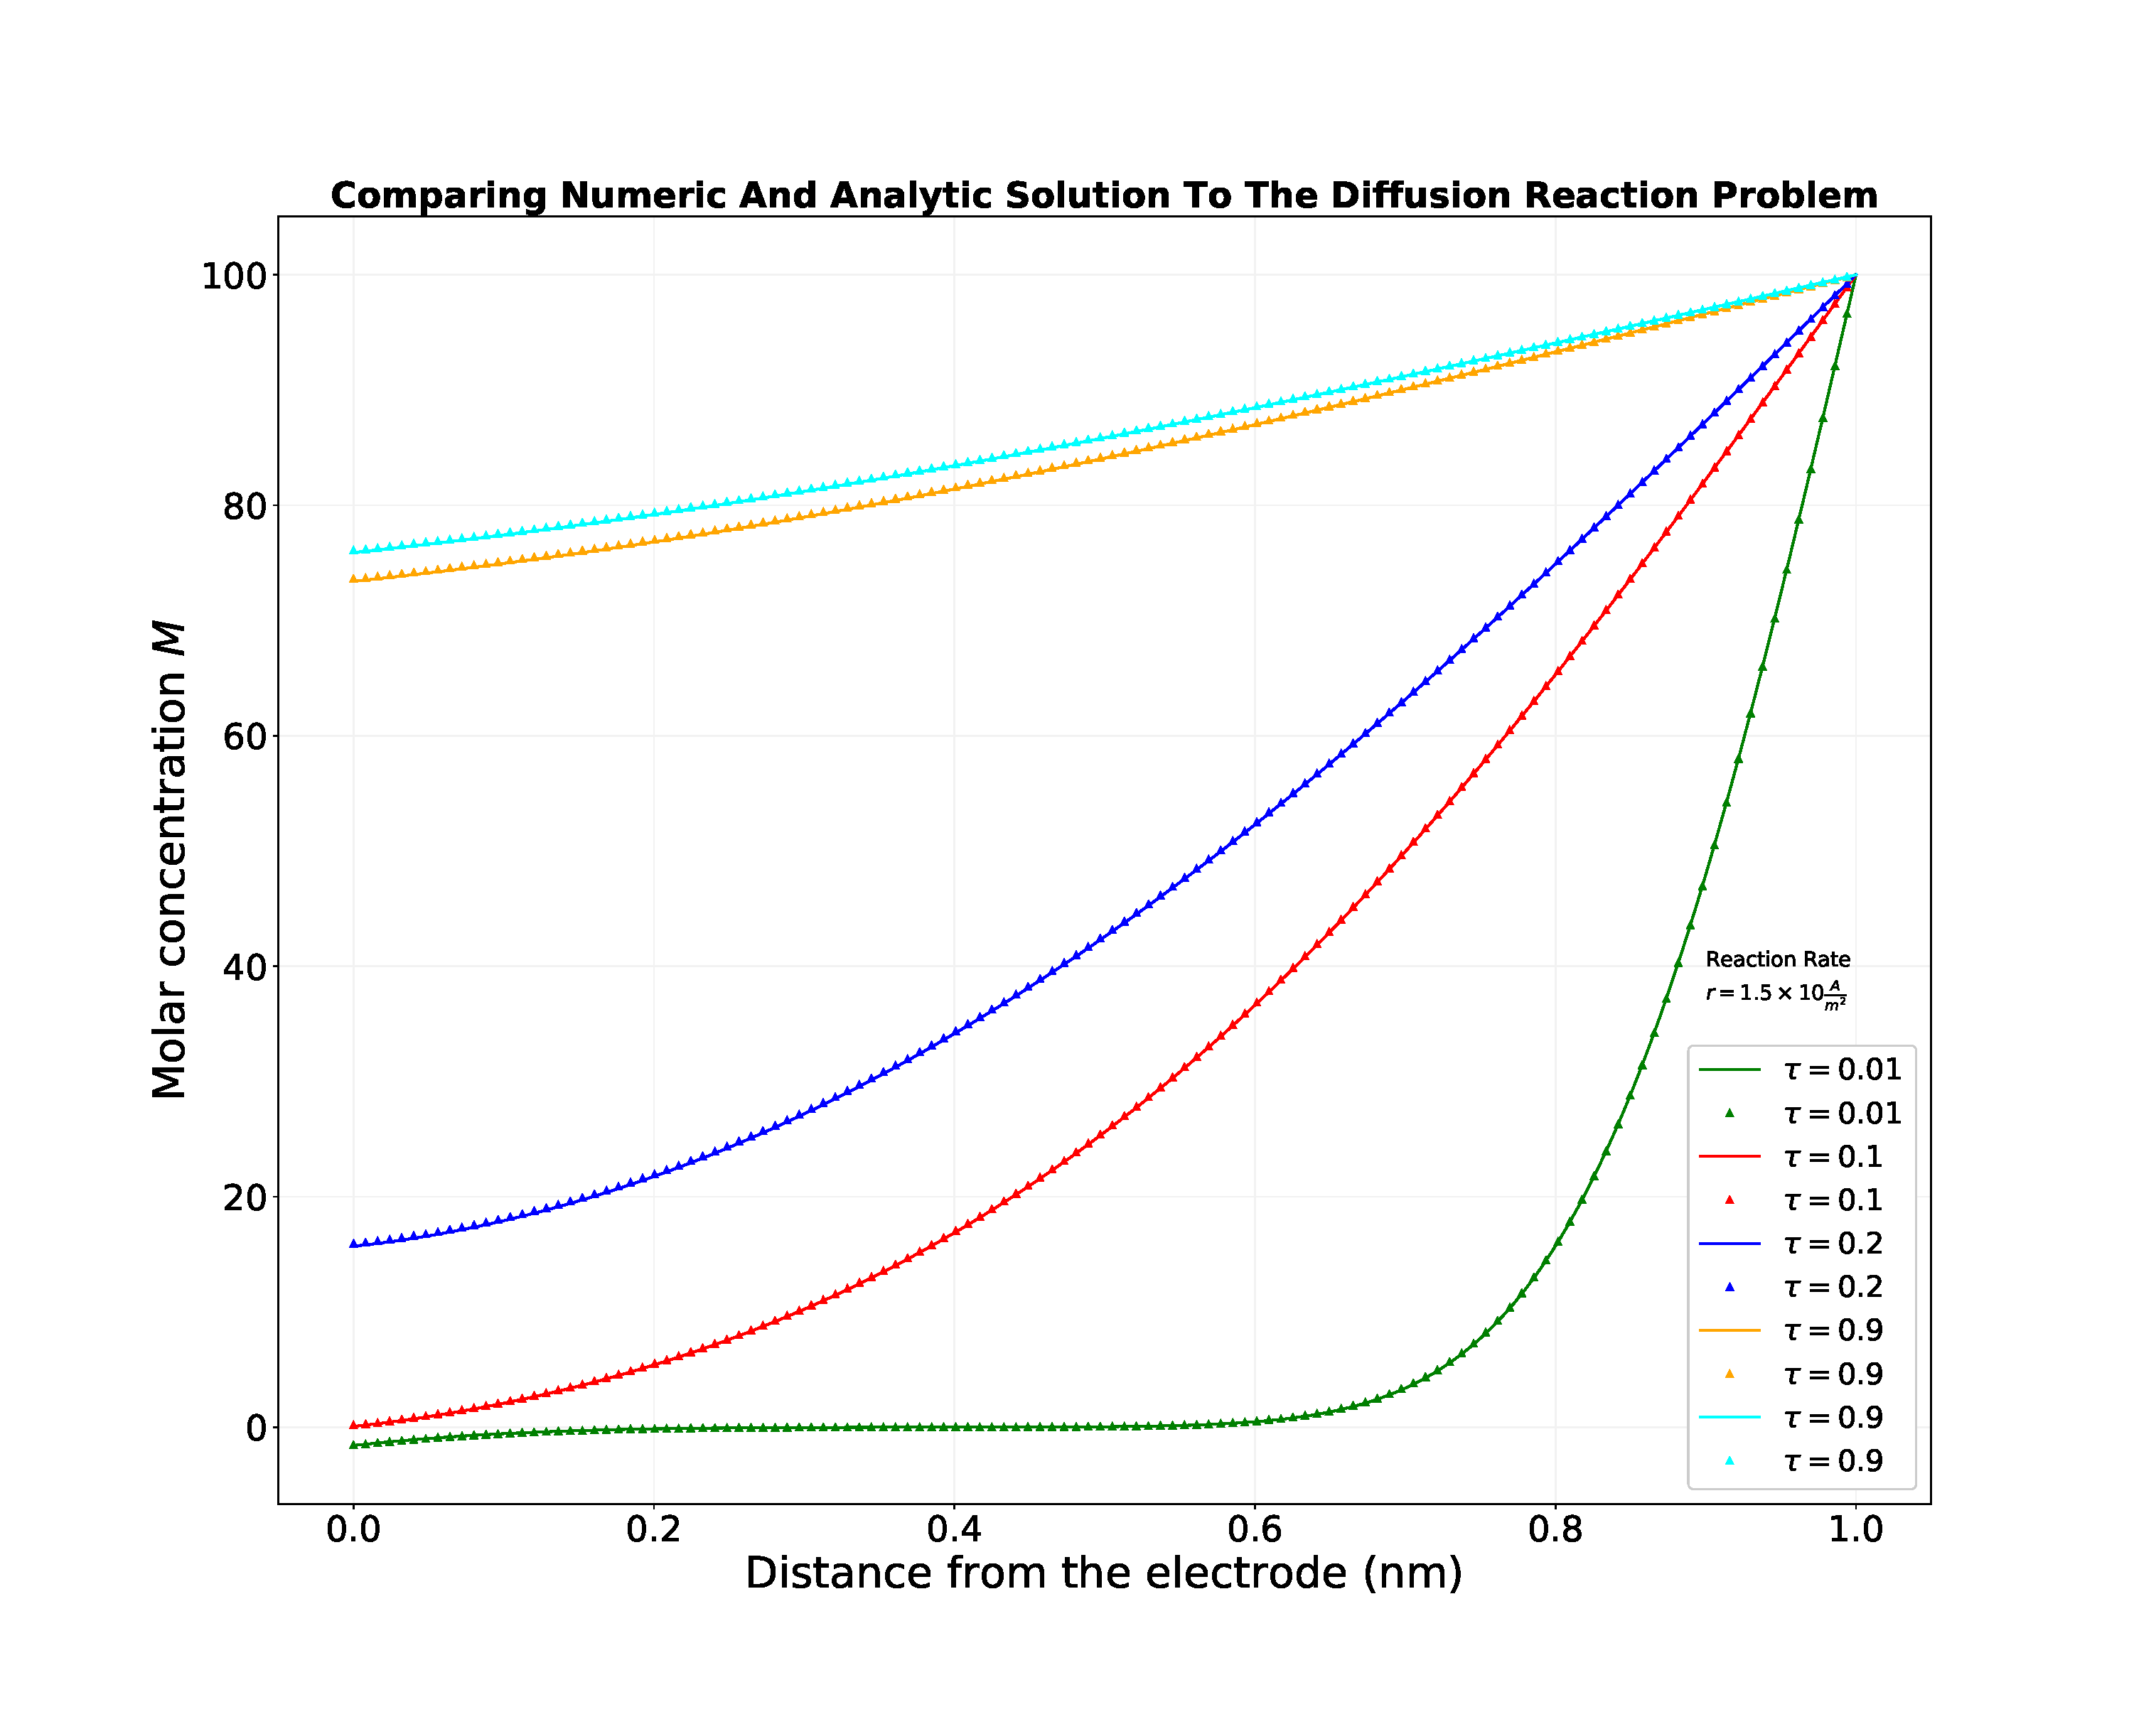
\includegraphics[width=\textwidth]{diffusion-reaction-comparison}
\caption{Each curve represents the concentration profile at increasingly large $t$. Continuos lines represent the analytic solution at each time step and the discrete markers listed in the image legend are represent the numerical solution. Steady State in the diffusion-only problem will be when concentration is $C_b=1$ throughout the domain.}
\label{fig:diffusion-reaction-comparison-fixed-r}
\end{figure}


